  \pagebreak
  \section{Actividad Práctica}
    Se propone realizar las mediciones de \textbf{potencias} y \textbf{factor de potencia}, y posteriormente,
    la \textbf{correción} de dicho factor, en una carga reactiva, la cual se trata de un tubo fluorescente 
    común. Este mismo se encuentra preparado junto a un circuito de medición que provee la cátedra. En la 
    Figura~\ref{fig:CircuitoMedicion} se puede apreciar un esquema del mismo y una foto real.

    \begin{figure}[H]
      \centering
        \begin{subfigure}[t]{0.7\textwidth}
          \centering
          \frame{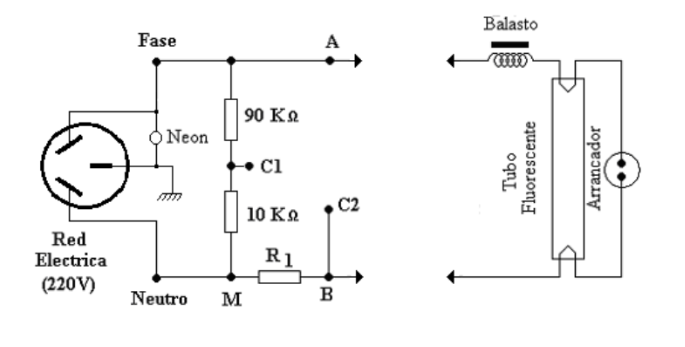
\includegraphics[width=\textwidth]{Imagenes/ActividadPractica/EsquemaCircuito.png}}
          \caption{Esquema.}
          \label{fig:EsquemaCircuito}
        \end{subfigure}
        \begin{subfigure}[t]{0.7\textwidth}
          \centering
          \frame{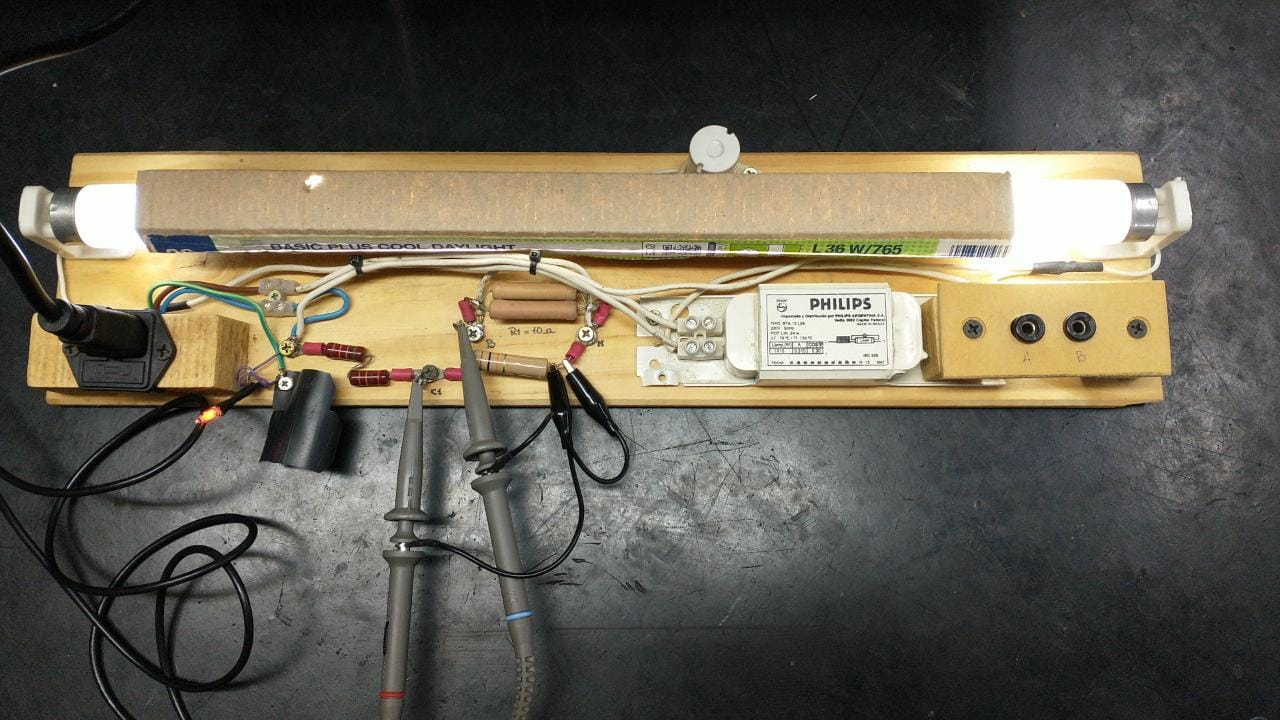
\includegraphics[width=\textwidth]{Imagenes/ActividadPractica/FotoRealCircuito.jpeg}}
          \caption{Foto real.}
          \label{fig:FotoRealCircuito}
        \end{subfigure}
      \caption{Circuito de medición propuesto por la cátedra.}
      \label{fig:CircuitoMedicion}
    \end{figure}

    En el circuito de medición se puede apreciar el punto \textbf{M}, en el cual se conecta la tierra del osciloscopio
    por medio de sus puntas. Por esta razón, es importante y obligatorio el uso de un \textbf{transformador de aislación},
    el cual tiene una de relación 1:1, y tiene como función crear una barrera física de aislación
    entre los equipos/circuitos con los cuales se trabaja y la red. Esto se justifica con que, la diferencia de
    potencial entre \textit{neutro} y \textit{tierra} de la red no es cero (idealmente debería serlo), para este caso, dicho
    valor es de aproximadamente $\mathbf{1,27\ V}$. Este valor generaría un flujo de corriente a través del osciloscopio 
    directo a la \textit{tierra}, lo cual podría dañar el instrumento, y además, provocaría que el diferencial se active.

    Siguiendo con el análisis del circuito de medición, se puede apreciar un divisor resistivo. Esto permite que, en el
    punto \textbf{C1} se pueda medir la \textbf{décima parte} de la tensión de entrada. Luego, en el punto \textbf{C2} 
    se mide la corriente de entrada por Ley de Ohm, ya que el valor de la resistencia es $\mathbf{R_1=10\ \Omega}$.
    
    Se aclara que el kit utilizado no respeta el código de colores de los cables, siendo la fase y el neutro de color azul
    y marrón respectivamente.

      \subsection{Medición de potencia activa y factor de potencia} 
  

      \subsection{Correción del factor de potencia}


